\documentclass{beamer}\usepackage[]{graphicx}\usepackage[]{color}
%% maxwidth is the original width if it is less than linewidth
%% otherwise use linewidth (to make sure the graphics do not exceed the margin)
\makeatletter
\def\maxwidth{ %
  \ifdim\Gin@nat@width>\linewidth
    \linewidth
  \else
    \Gin@nat@width
  \fi
}
\makeatother

\definecolor{fgcolor}{rgb}{0.345, 0.345, 0.345}
\newcommand{\hlnum}[1]{\textcolor[rgb]{0.686,0.059,0.569}{#1}}%
\newcommand{\hlstr}[1]{\textcolor[rgb]{0.192,0.494,0.8}{#1}}%
\newcommand{\hlcom}[1]{\textcolor[rgb]{0.678,0.584,0.686}{\textit{#1}}}%
\newcommand{\hlopt}[1]{\textcolor[rgb]{0,0,0}{#1}}%
\newcommand{\hlstd}[1]{\textcolor[rgb]{0.345,0.345,0.345}{#1}}%
\newcommand{\hlkwa}[1]{\textcolor[rgb]{0.161,0.373,0.58}{\textbf{#1}}}%
\newcommand{\hlkwb}[1]{\textcolor[rgb]{0.69,0.353,0.396}{#1}}%
\newcommand{\hlkwc}[1]{\textcolor[rgb]{0.333,0.667,0.333}{#1}}%
\newcommand{\hlkwd}[1]{\textcolor[rgb]{0.737,0.353,0.396}{\textbf{#1}}}%

\usepackage{framed}
\makeatletter
\newenvironment{kframe}{%
 \def\at@end@of@kframe{}%
 \ifinner\ifhmode%
  \def\at@end@of@kframe{\end{minipage}}%
  \begin{minipage}{\columnwidth}%
 \fi\fi%
 \def\FrameCommand##1{\hskip\@totalleftmargin \hskip-\fboxsep
 \colorbox{shadecolor}{##1}\hskip-\fboxsep
     % There is no \\@totalrightmargin, so:
     \hskip-\linewidth \hskip-\@totalleftmargin \hskip\columnwidth}%
 \MakeFramed {\advance\hsize-\width
   \@totalleftmargin\z@ \linewidth\hsize
   \@setminipage}}%
 {\par\unskip\endMakeFramed%
 \at@end@of@kframe}
\makeatother

\definecolor{shadecolor}{rgb}{.97, .97, .97}
\definecolor{messagecolor}{rgb}{0, 0, 0}
\definecolor{warningcolor}{rgb}{1, 0, 1}
\definecolor{errorcolor}{rgb}{1, 0, 0}
\newenvironment{knitrout}{}{} % an empty environment to be redefined in TeX

\usepackage{alltt}

%%%%%%%%%%%%%%%%%%%%%%%%%%%%%%%%%%%
%%% Beamer option
%%%%%%%%%%%%%%%%%%%%%%%%%%%%%%%%%%%
\usetheme{Madrid}
\usecolortheme{beaver}
\beamertemplatenavigationsymbolsempty
\setbeamertemplate{itemize item}[triangle]
\setbeamercolor{itemize item}{fg=red}
%%%%%%%%%%%%%%%%%%%%%%%%%%%%%%%%%%%

%%%%%%%%%%%%%%%%%%%%%%%%%%%%%%%%%%%
\usepackage{lmodern}
\usepackage[english]{babel}
\usepackage{natbib}


%%%%%%%%%%%%%%%%%%%%%%%%%%%%%%%%%%%
%% Hyperlinks
\usepackage{hyperref}
\hypersetup{colorlinks=true, urlcolor=blue}



%%%%%%%%%%%%%%%%%%%%%%%%%%%%%%%%%%%
%% Maths
\usepackage{amsmath,amsthm,amssymb,amsfonts}
\newcommand{\E}{\mathbb{E}}
\newcommand{\Var}{\mathbb{V}ar}

%%%%%%%%%%%%%%%%%%%%%%%%%%%%%%%%%%%
%% Tables
\usepackage{floatrow} %centre automatic les figures
\floatsetup[table]{capposition=top}
\usepackage{multirow}
\usepackage[toc,page]{appendix}

%%%%%%%%%%%%%%%%%%%%%%%%%%%%%%%%%%%
%% Figs
\usepackage{graphicx}
\usepackage{caption}
%\usepackage{subcaption}
\graphicspath{{./figure/}}
%%%%%%%%%%%%%%%%%%%%%%%%%%%%%%%%%%%
%% Verbatim code
%\usepackage{alltt}

%%%%%%%%%%%%%%%%%%%%%%%%%%%%%%%%%%%
%% Title page
\title{ggplot2 Introduction}
\author{Jean-Baptiste Lecomte}


%%%%%%%%%%%%%%%%%%%%%%%%%%%%%%%%%%%
%% Start documents
%%%%%%%%%%%%%%%%%%%%%%%%%%%%%%%%%%%
\IfFileExists{upquote.sty}{\usepackage{upquote}}{}
\begin{document}


\maketitle




%%%%%%%%%%%%%%%%%%%%%%%%%%%%%%%%%%%
%% Introduction
%%%%%%%%%%%%%%%%%%%%%%%%%%%%%%%%%%%
\begin{frame}{Introduction}
  \begin{itemize}
    \item developped by Hadley Wickham (Rice University, Houston, USA)
    \item highly recommanded R packages to work with ggplot2: reshape and plyr (also developped by H. Wickham)
    \item first version called in 2007
  \end{itemize}
\end{frame}

\begin{frame}{Useful books}
  \begin{columns}
    \begin{column}{0.5\textwidth}
      
\includegraphics[scale=0.45]{rgraphicscookbook}
    \end{column}
  
    \begin{column}{0.5\textwidth}
      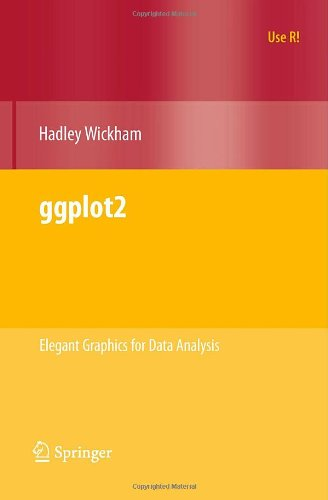
\includegraphics[scale=0.45]{ggplot2}
    \end{column}
  \end{columns}
\end{frame}

\begin{frame}{Online ressources}
    	\begin{itemize}
        \item R code related to ggplot2 cookbook:\\ \url{http://www.cookbook-r.com/Graphs/}
        \item R code related to useR! ggplot2 book:\\ \url{http://ggplot2.org/book/}
  		  \item ggplot2 official documentation:\\  \url{http://docs.ggplot2.org/current/}
			  \item Google groups to ask questions:\\ \url{ggplot2@googlegroups.com}
        \item Github repository:\\ \url{https://github.com/yhat/ggplot/}
			\end{itemize}
\end{frame}


\begin{frame}{Introduction}
  \begin{itemize}
    \item based on new aesthetic principles
    \item based on \textit{The grammar of graphics} developed by Wilkinson in 2005
    \item efficient way to produce simple graphics with a length reduction of R code
  \end{itemize}
  
  \begin{alertblock}{Forget about R base graphics:}
     \texttt{ plot(), hist(), par(), layout(), points(), lines(),legend()}
  \end{alertblock}
\end{frame}

\begin{frame}{Principle}
ggplot2 is based on a \textbf{layer} system which can be used as objects.\\
\vspace{1cm}
Main layers
  \begin{itemize}
    \item data $\rightarrow$ raw data
    \item mapping $\rightarrow$ graphic projection
    \item geom $\rightarrow$ geometric objects (points, lines, polygons, ...)
    \item stat $\rightarrow$ statistics transformation (histogram, model)
    \item scale $\rightarrow$ aesthetics customization (color, shape, size, axes, legend)
    \item coord $\rightarrow$ coordinate system (axes, grid)
    \item facet $\rightarrow$ subdivision (lattice, trellis)
  \end{itemize}
\end{frame}

\begin{frame}{Base functions}
ggplot2 is based on two functions:
  \begin{enumerate}
		\item  \texttt{qplot()} for \textbf{q}uick \textbf{plot}
		\begin{itemize}
			\item easy and fast, but too simple in most cases
			\item \texttt{qplot(x, y, data=data)}
		\end{itemize}
    \vspace{0.5cm}
    \item \texttt{ggplot()}
      	\begin{itemize}
			\item more complex but more powerful and flexible by adding \texttt{layers}
			\item \texttt{ggplot(data=data, aes(x, y)) + layers}
		\end{itemize}
  \end{enumerate}
\end{frame}


\begin{frame}[fragile]{Getting Started}

  \begin{alertblock}{Data format}
    Always work with a \texttt{data.frame}
  \end{alertblock}
    Our data frame:
    
\begin{knitrout}
\definecolor{shadecolor}{rgb}{0.969, 0.969, 0.969}\color{fgcolor}\begin{kframe}
\begin{alltt}
  \hlkwd{head}\hlstd{(df_data)}
\end{alltt}
\begin{verbatim}
##     Year Month DURATION_MINUTES AREA Avg_net_depth Avg_net_temp       Date
## 476 2005     7               21  5AB    -0.3162932     0.393884 2005-07-06
## 477 2005     7               20  5AB    -0.4353716     0.433940 2005-07-06
## 478 2005     7               21  5AB    -0.4418207     0.300420 2005-07-07
## 479 2005     7               21  5AB    -0.2340669     0.133520 2005-07-07
## 480 2005     7               20  5AB    -0.1713032    -0.026704 2005-07-07
## 481 2005     7               20  5AB    -0.1683089    -0.353828 2005-07-07
##          Lon    Lat        X       Y     X_km     Y_km Pres Year_fac
## 476 -127.970 51.160 572025.0 5668122 572.0250 5668.122    1     2005
## 477 -127.995 51.140 570307.2 5665874 570.3072 5665.874    1     2005
## 478 -128.225 51.610 553664.9 5717947 553.6649 5717.947    1     2005
## 479 -128.250 51.625 551916.7 5719597 551.9167 5719.597    1     2005
## 480 -128.330 51.665 546338.2 5723992 546.3382 5723.992    1     2005
## 481 -128.335 51.700 545956.9 5727882 545.9569 5727.882    1     2005
##     AREA_num nFish   Biomass
## 476        1     1  2.048385
## 477        1     5 11.630089
## 478        1     6 14.310041
## 479        1     7 17.350754
## 480        1     1  2.139599
## 481        1     3  7.909197
\end{verbatim}
\end{kframe}
\end{knitrout}
\end{frame}

%%%%%%%%%%%%%%%%%%%%%%%%%%%%%%%%%%%
%% Example
%%%%%%%%%%%%%%%%%%%%%%%%%%%%%%%%%%%

\begin{frame}[fragile]{Scatter plot: Depth and Biomass}
\begin{knitrout}
\definecolor{shadecolor}{rgb}{0.969, 0.969, 0.969}\color{fgcolor}\begin{kframe}
\begin{alltt}
  \hlstd{scatter.plot} \hlkwb{<-} \hlkwd{ggplot}\hlstd{(}\hlkwc{data}\hlstd{=df_data,} \hlkwd{aes}\hlstd{(}\hlkwc{x}\hlstd{=Avg_net_depth,}
                                           \hlkwc{y}\hlstd{=Biomass))} \hlopt{+}
                \hlkwd{geom_point}\hlstd{()}
  \hlkwd{print}\hlstd{(scatter.plot)}
\end{alltt}
\end{kframe}
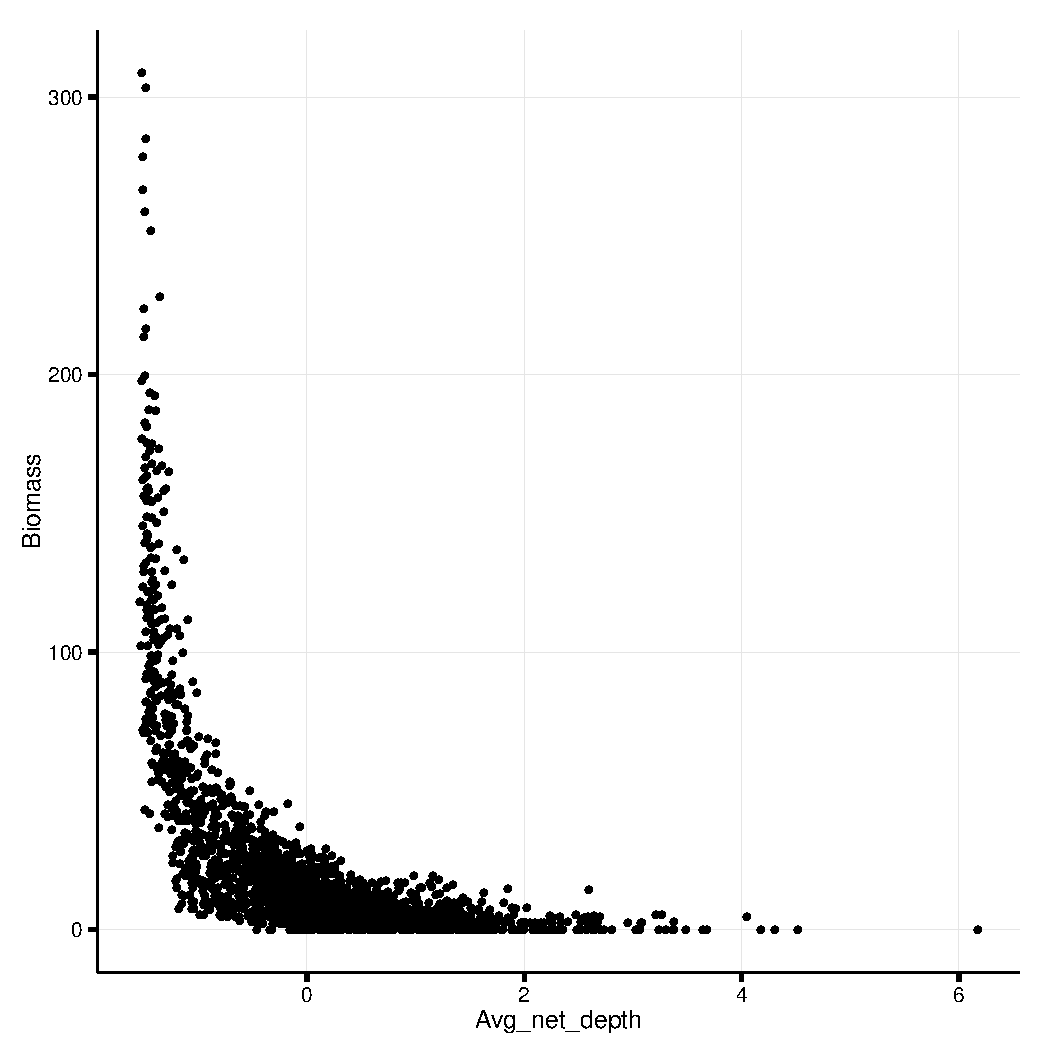
\includegraphics[width=\maxwidth]{boring-plot-1} 

\end{knitrout}
       
%<<boring-plots, dev=pdf, fig.width=5, fig.height=5, eval=FALSE, literal=TRUE>>=
%       scatter_plot
%       @
\end{frame}

\end{document}
